\documentclass[../qm.tex]{subfiles}
\begin{document}
Consider a general reaction
\begin{equation*}
	p+p\to H+q_1+q_2
\end{equation*}
Where $H$ is the Higgs boson which decays as usual into two $Z^0$ bosons which decay in electron-positron or muon-antimuon couples, and $q_1,q_2$ are hadron swarms.\\
The ideal objective is to measure the 4-momentum of all particles. For this various kinds of detectors are used
\section{Trackers}
Tracker detectors for charged particles which measure $p$ through ionization. They rebuild the trace of the particle and use the radius of curvature of the path and use it for finding $p$.\\
In this case $\dv{E}{x}$ must be measurable.\\
In order to have this reduction of $E$ from ionization we have from Bethe-Bloch that
\begin{equation*}
	-\dv{E}{x}\propto C\rho\frac{Z}{A}f(\beta\gamma)
\end{equation*}
Inside the detector we have that the reduction of energy is
\begin{equation*}
	-\dd E\propto\rho\dd x
\end{equation*}
And therefore we need $\rho$ small (i.e. a gas) and a thin $\dd x$
\subsection{Cloud Chambers}
Cloud chambers are a simple kind of tracker detector composed by a container filled with saturated vapor.\\
The charged particles passing through the vapor ionize it, creating bubbles around the ions. After that the track can be photographed and then the needed values can be measured.\\
This type of particle detector was used to discover the positron. In that cloud chamber a $6\unit{mm}$ thick slab of $\nuc{Pb}{}{}$ was used as a target to slow the particles and a magnetic field was applied.\\
\begin{figure}[H]
	\centering
	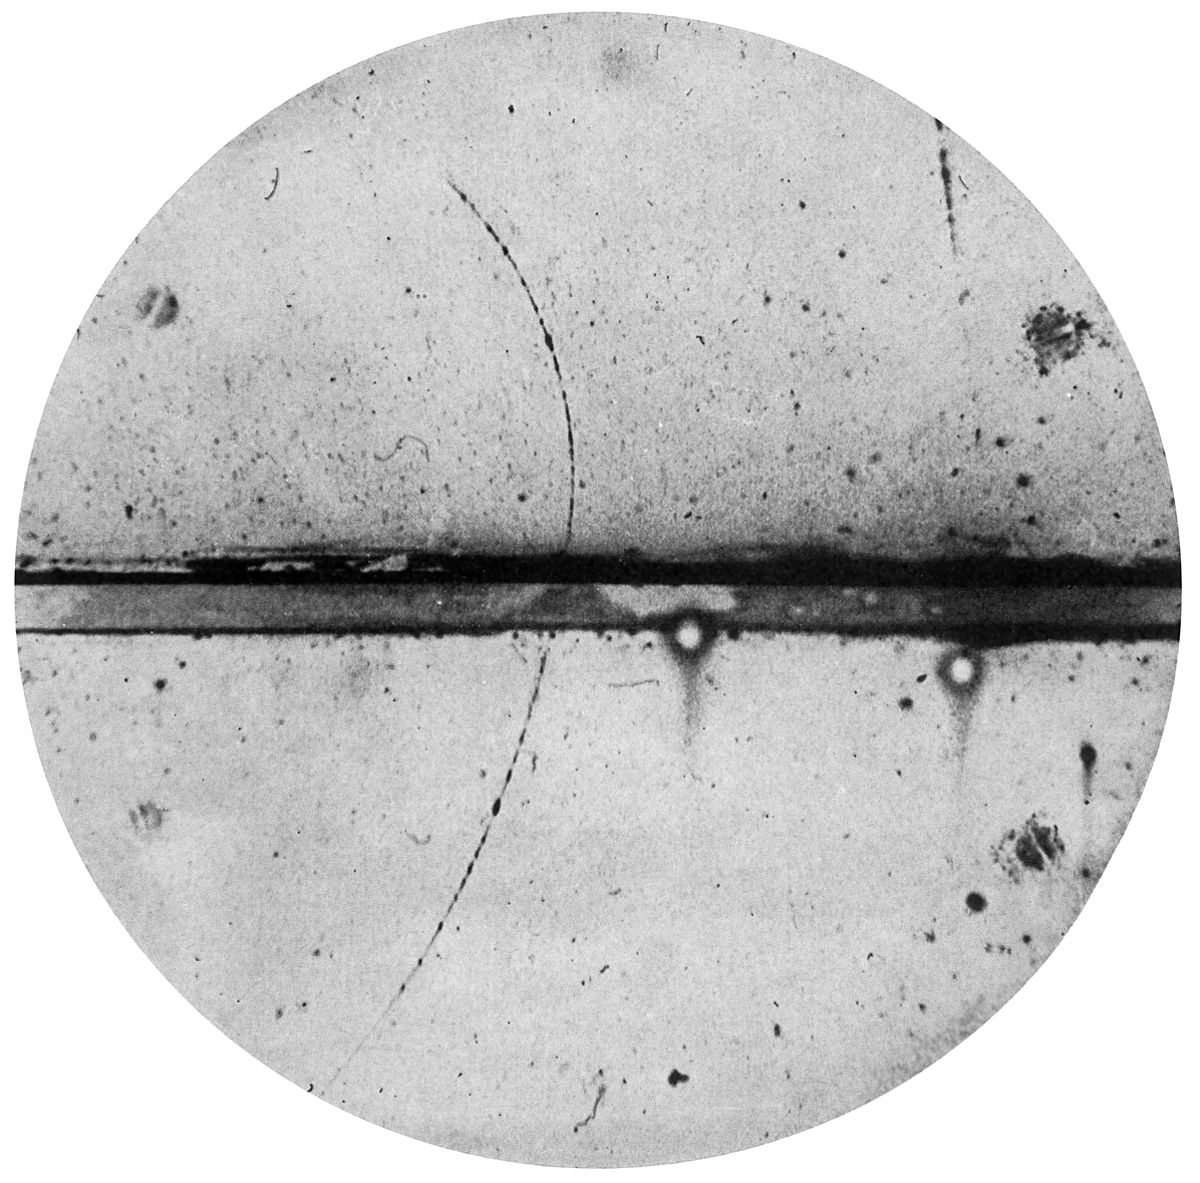
\includegraphics[keepaspectratio,width=\linewidth]{cchamber.jpg}
	\caption{The picture taken to the cloud chamber in 1932 by Anderson et al. that shown the production of a positron}
	\label{fig:positrondisc}
\end{figure}
From the photo it's possible to identify a particle going through the lead from the bottom, with $p_i=63\unit{MeV}$ and with $p_f=23\unit{MeV}$. Using $\chi_{0,\mathrm{Pb}}=5.6\unit{mm}$ we have that
\begin{equation*}
	E(\chi_0)\approx\frac{E_0}{3}
\end{equation*}
Supposing that the particle is a proton we would have
\begin{equation*}
	\beta\gamma=\frac{p}{m_p}=\frac{63}{1000}\approx0.06
\end{equation*}
Since it's clear from the experiment that the particle passed more than $6\unit{cm}$, we have that it must be an unknown particle, the positron in this case. Doing the same calculation with $m_e$ we get $\beta\gamma\approx120$.\\
A slight modification of this is the bubble chamber, which uses high pressure liquids to create the saturated vapor. This detector has a much greater spatial resolution with $\delta x\approx100\unit{\mu m}$
\subsection{Nuclear Emulsions}
Another kind of tracker detector used is the nuclear emulsion, where gelatinous slabs of silver bromide $\mathrm{AgBr}$ are in a suspension on the slab.\\
The ionization of charged particles releases electrons that make silver shine engraving the track permanently on the slab.\\
This type of detector has a resolution of $\delta x\approx1\unit{\mu m}$, but it's slow to analyze, and therefore it's useful for processes with low frequencies.
\section{Ionization Detectors}
Ionization detectors function by catching the ionization charge of the particles passing by. The measured signal depends on $\dv{E}{x}$ and on the potential difference $\Delta V$ created by two plates that enclose a noble gas.\\
Chapak in 1962 proposed the construction of such detector with cathode planes and parallel anode wires. The spectral resolution of such detector is $\delta x\approx300\unit{\mu m}$
\subsection{Drift Chambers}
Drift chambers are ionization detectors made by a multiwire proportional chamber which measures the time needed for a signal to arrive from one side to another
\subsection{Silicon Detectors}
Silicon detectors are another kind of ionization detectors. They are really quick and have a high resolution. They use semiconductors.\\
Considering that $\rho_{\mathrm{Si}}$ is big, the detectors are quite thin, with a resolution of $\delta x\approx10\unit{\mu m}$. Note that their resolution is deeply tied to the magnetic field $B$ and thickness of the detector $L$, in fact we have
\begin{equation}
	\frac{\delta P}{P}=\frac{P}{0.3BL^2}\delta x
	\label{eq:resolutionsilicondet}
\end{equation}
I.e., the resolution gets smaller when $P$ grows. Note that
\begin{equation*}
	P\approx0.3BR
\end{equation*}
Where $P$ is expressed in $\unit{GeV}$, $B$ in $\unit{T}$ and $R$ in $\unit{m}$
\section{Calorimeters and Energy Measures}
The passage of photons, electron positron pairs and hadrons creates EM or hadronic swarms inside mediums. Their ionization can excite molecules or atoms inside this medium.\\
One kind of calorimeter is the scintillator, which records the de-excitation photons of the swarms (in the visible, close UV spectra). There are two major kinds of scintillators
\begin{enumerate}
\item Organic or plastic scintillators made mainly from anthracene, with a response time of $10^{-8}\unit{s}$
\item Inorganic or crystalline scintillators, made mainly from $\mathrm{NaI, CsI, PbWO_4}$ with a response time of $10^{-6}\unit{s}$
\end{enumerate}
The main problem with scintillators is that the medium reabsorbs part of these de-excitation photons, giving fewer photons to measure, they activate mainly in the close UV region.\\
The main solution for solving the first problem is using doping materials in order to increase the scintillation photons.\\
\begin{figure}[H]
	\centering
	\begin{tikzpicture}
		\draw[->,decoration={complete sines, amplitude=2}, decorate] (-5,0) -- (-4,0);
		\node[below] at (-4.5,0) (g) {\tiny$\gamma$};
		\draw (-3.5,-0.3) rectangle (-1,0.3);
		\draw[pattern=north east lines] (-0.9,-0.3) rectangle (-0.6,0.3);
		\draw (-0.6,0.3) -- (3,0.3);
		\draw (-0.6,-0.3) -- (3,-0.3);
		\draw[pattern=north east lines] (3,-0.3) rectangle (3.3,0.3);
		\node[below] at (-0.64,-0.3) (fcath) {\tiny photocathode};
		\node[above] at (-2.24,0.3) (cry) {\tiny crystal};
		\node[right] at (3.3,0) (charge) {\tiny$q$ accumulator};
		\draw[->,thin] (-0.75,0) -- (0.5,0.3) -- (1,-0.3) -- (1.5,0.3) -- (2.3,-0.3) -- (3,0.2);
		\node[above] at (0.5,0.3) (e) {\tiny$e^-$};
		\draw[->,thin] (-1.5,0.15) -- (-1.1,0.15);
		\draw[->,thin] (-1.5,0) -- (-1.1,0);
		\draw[->,thin] (-1.5,-0.15) -- (-1.1,-0.15);
		\node[above] at (1.8,0.3) {\tiny photomultiplier};
	\end{tikzpicture}
	\caption{Tiny scheme describing how a scintillator functions}
	\label{fig:scintillator}
\end{figure}
As in the picture, the photocatode is a piece sensible to photons and photoelectric effects. It creates a landslide effects on diodes that amplify the photo-electron (photoelectric process' child particle).\\
For around 10 nodes it's possible to have a gain of $10^4$ till $10^7$ depending on the value of $\Delta V$. The charge measured $q$ is proportional to the number of photo-electrons and therefore proportional to the energy of the photons.\\
A detector made only of scintillators and photomultipliers is known as a \emph{homogeneous calorimeter}.\\
The calorimeters use long crystals, such that $N\chi_0\approx20\chi_0$ in order to contain more or less all the energy of the EM swarm. Therefore, for a crystal with $\chi_0=3\unit{cm}$ in a scintillator it'd be long at least $50\unit{cm}$.\\
Hadronic swarms, on the counterpart are regulated by the interaction length $\lambda>>\chi_0$, therefore using homogeneous calorimeters would be prohibitive since they'd need to be really long.\\
For hadrons usually \emph{sample calorimeters} which use a first scintillator block and multiple absorbent blocks, permitting an absorption of the hadrons, since $\lambda^{-1}=\rho\sigma$. Inside the absorber the swarm develops faster and we have
\begin{equation*}
	\delta q\propto\sqrt{N}\propto\sqrt{N}
\end{equation*}
In calorimeters we have
\begin{equation}
	\frac{\delta E}{E}\approx\frac{a}{\sqrt{E}}
	\label{eq:calresol}
\end{equation}
Where $a$ is a measured constant depending on the calorimeter used. This constant is known as the characteristic constant of the calorimeter, and it's known that $a_{hom}<a_{sample}$.\\
Note also that a higher energy input grants a better resolution, as clear from \eqref{eq:calresol}
\section{Particle Accelerators}
A great example, and the first, of particle accelerators, is the well known cathodic tube, which accelerates electrons using a variation of tension. It's a typical example of linear accelerator.\\
Other famous linear accelerators are PEP-II and BaBAR which managed to reach a $\sqrt{s}=90\unit{GeV}$
\subsection{Cyclotrons}
Cyclotron accelerators are a type of accelerators which use a magnetic field in order to accelerate circularly charged particles. It was first suggested by Lawrence in 1959 and accelerate ions emitted at the center of a circular object composed by two semicircular ``Dee''.\\
The frequency of a cyclotron is readily calculable using classical electromagnetism, and it's equal to
\begin{equation}
	\nu_c=\frac{qB}{2\pi m}
	\label{eq:cyclotronfreq}
\end{equation}
This comes since inside the cyclotron there is an uniformly accelerated circular motion caused by $\Delta V$. Using Newton's second law we have
\begin{equation*}
	F=ma=m\frac{v^2}{r}=qvB\implies{}\frac{v}{r}=\frac{qB}{m}
\end{equation*}
The period of a revolution is fixed by $B$, and equals
\begin{equation*}
	\Delta T=\frac{1}{\nu_c}=\frac{2\pi m}{qB}
\end{equation*}
Note that this formula is not relativistic. In the relativistic formulation, using $\Delta t=\gamma\delta\tau$ we have
\begin{equation}
	\nu_c=\frac{qB}{2\pi\gamma m}\qquad\gamma=\frac{E}{m}
	\label{eq:relcycfreq}
\end{equation}
It's quick to see that the cyclotron frequency depends on the velocity of the particle (in the relativistic case), and therefore ultrarelativistc $e^-$ are not suitable for a cyclotron.\\
Ions, being much heavier and slower, are a better particle candidate for use inside cyclotrons.\\
We have
\begin{equation*}
	T_{max}=\frac{1}{2}mv_{max}^2=\frac{1}{2}m\omega^2r^2
\end{equation*}
And therefore, setting $r=R$ with $R$ being the radius of the cyclotron, we get that the maximum kinetic energy reached by the ions inside the cyclotron is
\begin{equation}
	T_{max}=\frac{(qBR)^2}{2m}
	\label{eq:cycmaxtion}
\end{equation}
For relativistic particles, since if $v$ grows $1/\gamma$ decreases, we might suppose to decrease the cyclotron's frequency in order to keep valid the previous relation, keeping $B$ constant\\
This kind of variable-frequency cyclotron is known as a synchro-cyclotron, which use variable $E$ fields to reach this result.\\
Another solution is to variate $B$ while keeping $\nu_c$ constant in order to compensate for $\gamma^{-1}$, these accelerators are known as synchrotrons.\\
%In the ultrarelativistic limit $p=\gamma mv\approx\gamma mc$ we have that $qBR\approx\gamma mc=p$.\\
%For synchrocyclotrons we have that $qBR\approx p\approx0.3BR$, and using a $10\unit{m}$ radius synchrocyclotron with a $1\unit{T}$ magnetic field we have that
Synchrocyclotrons are usually used for accelerating particles from $10$ to $900\unit{MeV}$, which is a relatively small acceleration
\subsection{Synchrotrons}
Synchrotrons are the relativistic counterpart of cyclotrons. They work by fixing the radius $R$ and variating $B$ for compensating for $\gamma^{-1}$ in the synchrotron frequency formula
\begin{equation}
	\nu_s=\frac{qB}{2\pi\gamma m}
	\label{eq:synchrotronfreq}
\end{equation}
This kind of accelerator doesn't need to create poles like the cyclotrons and its ``Dees'' and a uniform $B$ field is not needed in all the accelerator, therefore there are multiple dipoles along the synchrotrons.\\
The principal limit of synchrotron is Larmor radiation, also known as synchrotron radiation, with power
\begin{equation}
	P_L=\frac{e^2}{6\pi\epsilon_0c^3}\gamma^4aP 2
	\label{eq:synchrad}
\end{equation}
Using $\gamma=E/m$ and $p=v^2/R$ we get
\begin{equation}
	P_L=\frac{e^2E^4}{6\pi\epsilon_0R^2m^4}
	\label{eq:synchrad2}
\end{equation}
Which, for a period $\Delta T=2\pi R/c$ gives that the energy lost in synchrotron radiation is
\begin{equation*}
	\Delta E_{lost}\propto\frac{E^4}{m^4R^2}
\end{equation*}
In order to balance this energy loss it's needed to make bigger synchrotrons. The biggest (so far) is the Large Hadron Collider in Geneva, a synchrotron with $R=4.3\unit{km}$. For electrons in the LHC ($m_e\approx500\unit{keV}$) we have that the lost energy is proportional to
\begin{equation}
	\Delta E_{e,LHC}\approx88.5\frac{E^4}{4300}
	\label{eq:energylosslhce}
\end{equation}
Which imposes that for high energy electrons all energy is used to compensate for radiative losses inside the synchrotron.\\
For LEP@CERN, an experiment lasted from 1988 till the early 2000, there was $\sqrt{s}=90\unit{GeV}$, for a single beam energy of $45\unit{GeV}$. It used the same tunnel of LHC and its radiative losses per lap were
\begin{equation*}
	\Delta E_{LEP}=84\unit{MeV/lap}
\end{equation*}
Note that
\begin{equation*}
	\nu_{LEP}=\frac{c}{2\pi R}=\frac{c}{27\unit{km}}\approx10^6\unit{Hz}
\end{equation*}
Note that for what we have seen it's impossible to accelerate electrons to $\unit{TeV}$ ranges without increasing the radius of the synchrotron. From 2000 onwards, using protons, a $\sqrt{s}=13\unit{TeV}$ has been reached, which corresponds to $6.5\unit{MeV}$ per beam.\\
A new project is planned, the FCC, a supercollider with a circumference of $100\unit{km}$ built in Geneva. With these radius it's possible to reach $\sqrt{s}=50\unit{TeV}$.
\end{document}
